In this section we present the ambisonics microphone array geometries used in the subsequent numerical simulations.
In both cases described below, the listener traverses a straight line away from the microphone(s), which will allow us to explore any dependence on source azimuth relative to the direction of travel (see \secref{sec:06_Simulation_Framework:Azimuth_Dependence}).

\subsection{Single-microphone array}\label{sec:06_Simulation_Framework:Point_Geometry}
Consider a single-microphone array geometry, illustrated in \figref{fig:06_Simulation_Framework:Point_Geometry}, in which a single ambisonics microphone ($P = 1$) is separated from the origin by a distance $u$ and placed along the longitudinal $x$-axis, such that its position is given by $\vec{u}_1 = (u,0,0)$.
(Recall that, according to our coordinate system described in \secref{sec:02_Acoustical_Theory:Coordinate_System}, the $+x$-axis points forward from the listener, the $+y$-axis points to the left, and the azimuth $\phi$ measures the angle away from straight ahead.)
In this configuration, we define the \textit{navigable region} as the segment of the $x$-axis connecting the origin and microphone position, i.e., all listener positions $\vec{r}_0 = (x_0, 0, 0)$ where $x_0 \in [0,u]$.

% Diagram of source/mic positions
\begin{figure}[t]
\centering
  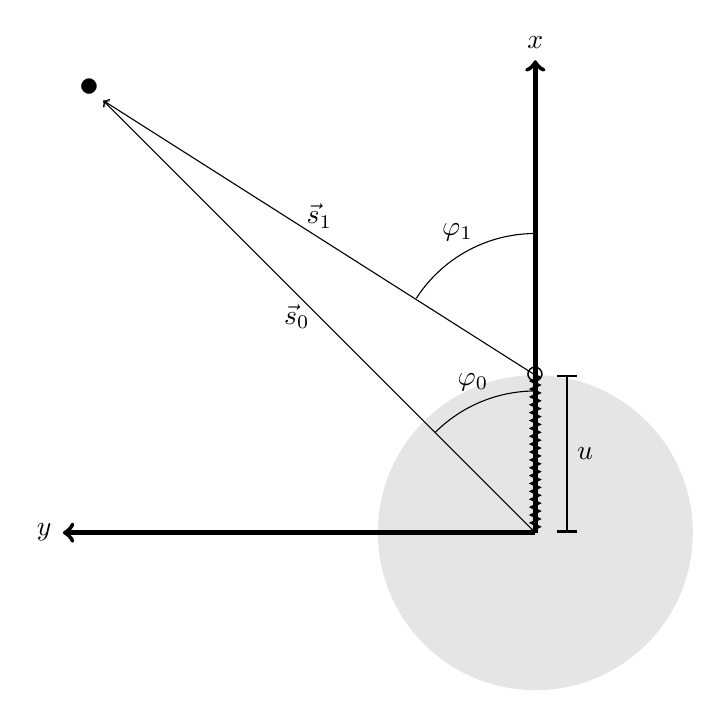
\begin{tikzpicture}[scale=4]
% Parameters
\def\radius{1.5};
\def\arrowScale{0.97};

\def\micSpacing{1};
\def\micL{-0.5*\micSpacing};

\def\sourceRadius{2};
\def\sourceAzimuth{45}
\pgfmathsetmacro\sourceY{cos(-\sourceAzimuth)*\sourceRadius}
\pgfmathsetmacro\sourceX{sin(-\sourceAzimuth)*\sourceRadius}

\pgfmathsetmacro\sourceLAzimuth{-atan(\sourceX/(\sourceY+\micL))}

\def\arcRadius{0.45};
\pgfmathsetmacro\arcY{cos(-\sourceAzimuth/2)*\arcRadius}
\pgfmathsetmacro\arcX{sin(-\sourceAzimuth/2)*\arcRadius}
\pgfmathsetmacro\arcLY{cos(-\sourceLAzimuth/2)*\arcRadius}
\pgfmathsetmacro\arcLX{sin(-\sourceLAzimuth/2)*\arcRadius}

% Coordinate system
\draw[ultra thick,->] (0,0) -- (0,\radius) node[above]{$x$};
\draw[ultra thick,->] (0,0) -- (-\radius,0) node[left]{$y$};

% Arrows
\node at (\sourceX,\sourceY){\Large $\bullet$}; % source
\draw[->] (0,0) -- (\arrowScale*\sourceX,\arrowScale*\sourceY) node[left, pos=0.5]{$\vec{s}_0$}; % origin
\draw[->] (0,-\micL) -- (\arrowScale*\sourceX,\arrowScale*\sourceY) node[above, pos=0.5]{$\vec{s}_1$}; % mic
\draw[thick, decoration = {zigzag, segment length = 1mm, amplitude = 0.5mm}, decorate] (0,0) -- (0,-\micL); % navigable region

% Arcs
\draw[domain=90:(90+\sourceAzimuth)] plot ({\arcRadius*cos(\x)}, {\arcRadius*sin(\x)});
\node at (1.15*\arcX,1.15*\arcY){$\varphi_0$};

%\draw[dashed,->] (\micL,0) -- (\micL,\arcRadius); % left mic
\draw[domain=90:(90+\sourceLAzimuth)] plot ({\arcRadius*cos(\x)}, {\arcRadius*sin(\x) - \micL});
\node at (1.15*\arcLX,1.15*\arcLY - \micL){$\varphi_1$};

% Mic positions
\node at (0,-\micL){\Large $\circ$};
\draw[thick,|-|] (0.1,0) -- (0.1,-\micL) node[right, pos=0.5]{$u$};

\fill [color=black,opacity=0.1] (0,0) circle (\micSpacing/2);

\end{tikzpicture}
  \caption[Diagram of the array geometry for extrapolation simulations.]{
  Diagram of a microphone (empty circle) and a single source (filled circle).
  The shaded gray disk indicates the interior region, where $r < u$.
  The jagged line segment indicates the navigable region, where $x \in [0,u]$ and $y = z = 0$.}
  \label{fig:06_Simulation_Framework:Point_Geometry}
\end{figure}

A single point source is placed on the horizontal plane at $\vec{s}_0 = (s_0 \cos \varphi_0, s_0 \sin \varphi_0, 0)$.
From the position of the microphone, the apparent source position is given by
$\vec{s}_1 = \vec{s}_0 - \vec{u} = (s_1 \cos \varphi_1, s_1 \sin \varphi_1, 0)$,
such that the apparent source azimuth is $\varphi_1$ and the relative source distance from the microphone is $s_1$.

We further define a nondimensional geometrical parameter $\gamma = r / u$.
Here we refer to the region with $\gamma > 1$ as the \textit{exterior region} and that with $\gamma < 1$ as the \textit{interior region} (see \figref{fig:06_Simulation_Framework:Point_Geometry}).

\subsection{Linear microphone array}\label{sec:06_Simulation_Framework:Linear_Geometry}
Consider a linear microphone array geometry, illustrated in \figref{fig:06_Simulation_Framework:Linear_Geometry}, in which a pair of ambisonics microphones ($P = 2$) are separated by a distance $\Delta = 2u$, equidistant from the origin and placed along the lateral $y$-axis, such that their positions are given by $\vec{u}_1 = (0,\Delta/2,0)$ and $\vec{u}_2 = (0,-\Delta/2,0)$.
In this configuration, we define the \textit{navigable region} as the segment of the $y$-axis connecting the two microphone positions, i.e., all listener positions $\vec{r}_0 = (0, y_0, 0)$ where $y_0 \in [-\Delta/2,\Delta/2]$.
Here also we define the same nondimensional geometrical parameter, now given by $\gamma = r / (\Delta / 2) = r / u$.

% Diagram of source/mic positions
\begin{figure}[t]
\centering
  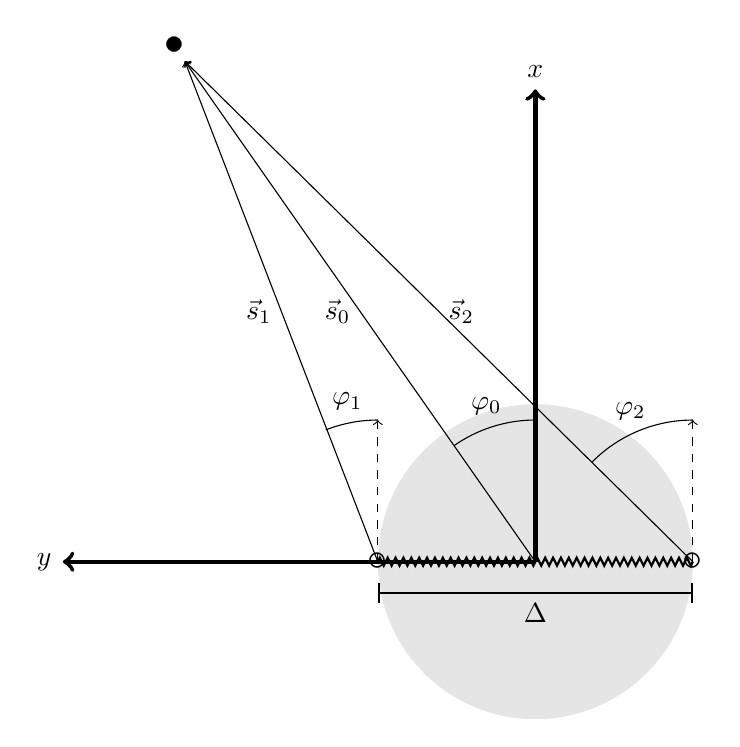
\begin{tikzpicture}[scale=4]
% Parameters
\def\radius{1.5};
\def\arrowScale{0.97};

\def\micSpacing{1};
\def\micL{-0.5*\micSpacing};
\def\micR{0.5*\micSpacing};

\def\sourceRadius{2};
\def\sourceAzimuth{35}
\pgfmathsetmacro\sourceY{cos(-\sourceAzimuth)*\sourceRadius}
\pgfmathsetmacro\sourceX{sin(-\sourceAzimuth)*\sourceRadius}

\pgfmathsetmacro\sourceLAzimuth{-atan((\sourceX-\micL)/\sourceY)}
\pgfmathsetmacro\sourceRAzimuth{-atan((\sourceX-\micR)/\sourceY)}

\def\arcRadius{0.45};
\pgfmathsetmacro\arcY{cos(-\sourceAzimuth/2)*\arcRadius}
\pgfmathsetmacro\arcX{sin(-\sourceAzimuth/2)*\arcRadius}
\pgfmathsetmacro\arcLY{cos(-\sourceLAzimuth/2)*\arcRadius}
\pgfmathsetmacro\arcLX{sin(-\sourceLAzimuth/2)*\arcRadius}
\pgfmathsetmacro\arcRY{cos(-\sourceRAzimuth/2)*\arcRadius}
\pgfmathsetmacro\arcRX{sin(-\sourceRAzimuth/2)*\arcRadius}

% Coordinate system
\draw[ultra thick,->] (0,0) -- (0,\radius) node[above]{$x$};
\draw[ultra thick,->] (0,0) -- (-\radius,0) node[left]{$y$};

% Arrows
\node at (\sourceX,\sourceY){\Large $\bullet$}; % source
\draw[->] (0,0) -- (\arrowScale*\sourceX,\arrowScale*\sourceY) node[left, pos=0.5]{$\vec{s}_0$}; % origin
\draw[->] (\micL,0) -- (\arrowScale*\sourceX,\arrowScale*\sourceY) node[left, pos=0.5]{$\vec{s}_1$}; % left mic
\draw[->] (\micR,0) -- (\arrowScale*\sourceX,\arrowScale*\sourceY) node[right, pos=0.5]{$\vec{s}_2$}; % right mic
\draw[thick, decoration = {zigzag, segment length = 1mm, amplitude = 0.5mm}, decorate] (\micL,0) -- (\micR,0); % navigable region

% Arcs
\draw[domain=90:(90+\sourceAzimuth)] plot ({\arcRadius*cos(\x)}, {\arcRadius*sin(\x)});
\node at (1.15*\arcX,1.15*\arcY){$\varphi_0$};

\draw[dashed,->] (\micL,0) -- (\micL,\arcRadius); % left mic
\draw[domain=90:(90+\sourceLAzimuth)] plot ({\arcRadius*cos(\x) + \micL}, {\arcRadius*sin(\x)});
\node at (1.15*\arcLX + \micL,1.15*\arcLY){$\varphi_1$};

\draw[dashed,->] (\micR,0) -- (\micR,\arcRadius); % right mic
\draw[domain=90:(90+\sourceRAzimuth)] plot ({\arcRadius*cos(\x) + \micR}, {\arcRadius*sin(\x)});
\node at (1.15*\arcRX + \micR,1.15*\arcRY){$\varphi_2$};

% Mic positions
\node at (\micL,0){\Large $\circ$};
\node at (\micR,0){\Large $\circ$};
\draw[thick,|-|] (\micL,-0.1) -- (\micR,-0.1) node[below, pos=0.5]{$\Delta$};

\fill [color=black,opacity=0.1] (0,0) circle (\micSpacing/2);

\end{tikzpicture}
  \caption[Diagram of the array geometry for interpolation simulations.]{
  Diagram of a two-microphone array (empty circles) with a single source (filled circle).
  The shaded gray disk indicates the interior region, where $r < \Delta / 2$.
  The jagged line segment indicates the navigable region, where $y \in [-\Delta/2,\Delta/2]$ and $x = z = 0$.}
  \label{fig:06_Simulation_Framework:Linear_Geometry}
\end{figure}

Similar to the single-microphone case, the apparent source position from the position of the $p^\textrm{th}$ microphone is given by
$\vec{s}_p = \vec{s}_0 - \vec{u}_p = (s_p \cos \varphi_p, s_p \sin \varphi_p, 0)$,
such that the apparent source azimuth is $\varphi_p$ and the relative source distance from that microphone is $s_p$.